
\begin{figure}[H]
\begin{center}
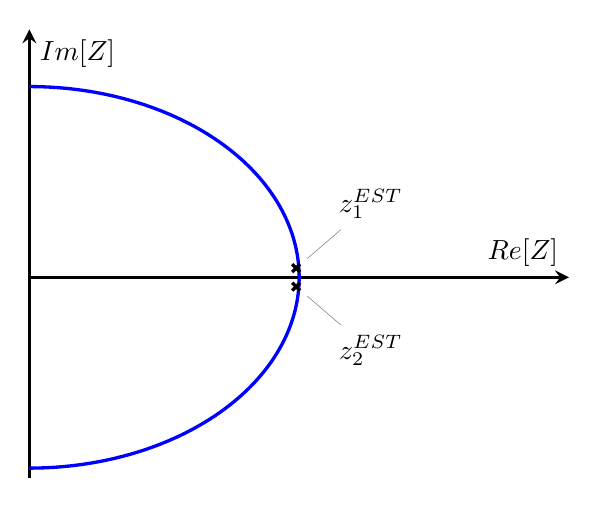
\begin{tikzpicture} 
\begin{axis}[very thick,
                     samples = 100,
                     ytick={-10,10},
                     xlabel = {$Re[Z]$},
                     ylabel = {$Im[Z]$},
                     xmin = 0,
                     xmax = 2,
                     ymin = -1.05,
                     ymax = 1.3,
                     axis x line = middle,
                     axis y line = middle,
                     ticks = none]
            \addplot [domain=-180:180, samples=1000, color=blue] ({cos(x)},{sin(x)});
            \addplot[mark=x] coordinates {(0.988862,0.0484835)} node[pin=50:{$z_{1}^{EST}$}]{};
            \addplot[mark=x] coordinates {(0.988862,-0.0484835)} node[pin=-50:{$z_{2}^{EST}$}]{};
        \end{axis}
        
\end{tikzpicture}
\end{center}
\caption{Círculo unitário para o sistema estável.}
\label{graph:1} 
\end{figure}
